%\documentclass[article,shortnames,nojss]{jss}
\documentclass{article}
\usepackage{graphicx}
\usepackage{url}
\usepackage{amssymb}
\usepackage{amsmath}
\usepackage{verbatim}
\usepackage{tikz}
\usepackage{rotating}

\usetikzlibrary{positioning,petri}

%\VignetteIndexEntry{Multiple table data in R}
%\VignettePackage{multitable}
%\VignetteDepends{multitable, MASS}
%\VignetteKeywords{data manipulation, ecology, multivariate, R}


%%%%R commands for running Sweave%%%%%%%
%%%%setwd("/users/stevenwalker/documents/multitable/multitable/vignettes/readingmultipletables/")
%%%%Sweave("/users/stevenwalker/documents/multitable/multitable/vignettes/readingmultipletables/readingmultipletables.Rnw")

\newcommand{\R}{{\sf R}}
\newcommand{\code}[1]{\texttt{#1}}
\title{Multiple-table data in \R}
\author{SC Walker}

\newcounter{exercise}
\numberwithin{exercise}{section}
\newcommand{\exnumber}{\addtocounter{exercise}{1} \theexercise \thinspace}

\usepackage{Sweave}
\begin{document}
\maketitle

The standard data management paradigm in \R\ is based on \code{data.frame} objects, which are two-dimensional data tables with rows and columns representing replicates and variables respectively.  Standard \R\ workflows require that all of the data to be analyzed is organized into a single data frame, and hypotheses about the relationships between variables in the data frame are expressed using \code{formula} objects; data frames and formulas are combined by passing them to functions that produce analyses (e.g. plots; fitted models; summary statistics).  This framework allows ecologists to concentrate on their primary interests---the relationships between ecological variables---without explicit reference to complex mathematical and algorithmic details.  It also provides access to those details, which are required (1) for more effective analyses and (2) to develop new methods of analysis within the framework.  As new methods are developed, researchers simply pass their data frames to new functions in much the same way they would pass them to older functions.  Thus, by separating low-level methods development from high-level data analysis, \R\ fosters the formation of a community of researchers where both methodologists and analysts can have mutually beneficial interactions.

However, research in my field of community ecology has led me to data sets that do not easily fit within a single data frame.  A common example is the fourth-corner problem (Legendre et al. 1997), in which three data tables are to be analyzed: a sites-by-species table of abundances or occurrences; a table of environmental variables at each site; and a table of traits for each species (Fig. \ref{fig:fourth}).  Such data are characterized by a conspicuous (lower-right) `fourth-corner', where there are no data.  These fourth-corners of missing data are not caused by the usual problems (e.g. broken field equipment; budget restrictions; bad weather; dead subjects), but are part of the study design itself.  The fourth-corner problem is a special case of a general `multiple-table problem', which can be much more complex (e.g. could involve three-dimensional `cubes' of data, Fig. \ref{fig:beatrix}).  The challenge of analyzing such multiple-table data sets in \R\ is that it is not obvious how to organize them into a single\code{data.frame}, which is required in standard \R\ workflows.  Our goal with the \code{multitable} package is to provide tools for analyzing multiple-table data sets within this standard \R\ framework.

\begin{figure}
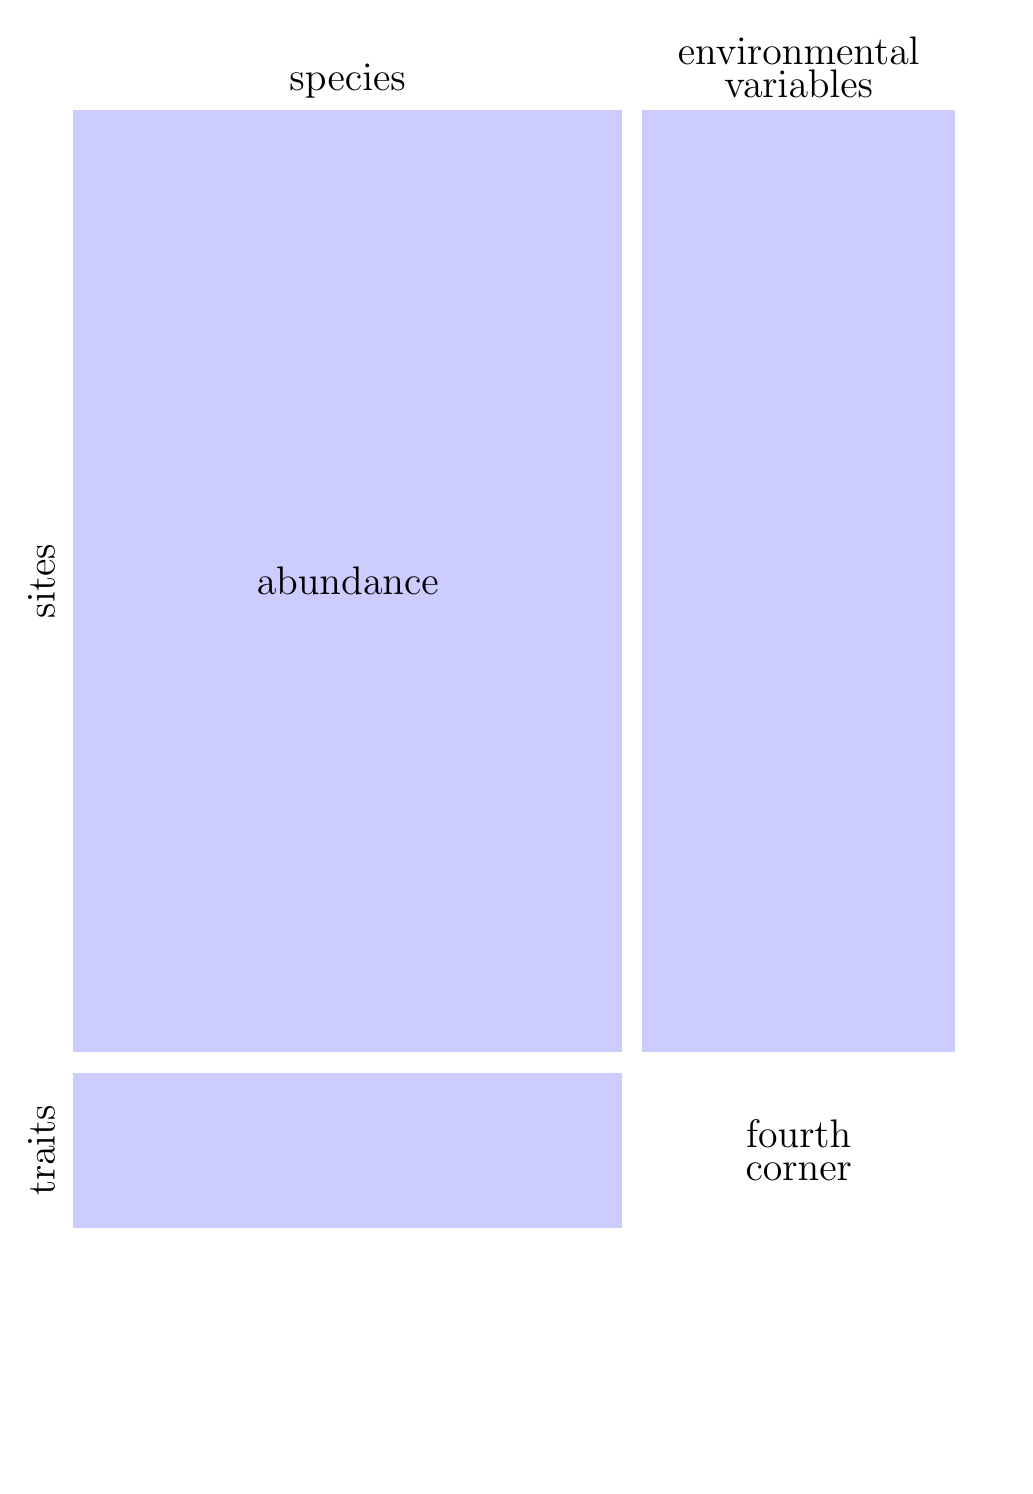
\begin{tikzpicture} [
	text centered,
	node distance=0.2cm,
	Y/.style={
		rectangle,draw=blue!0,fill=blue!20,thick,
		minimum width=7cm,minimum height=12cm,
		label=above:\Large species},
	X/.style={
		rectangle,draw=blue!0,fill=blue!20,thick,
		minimum width=4cm,minimum height=12cm,
		label={
		[text width=5cm]above:\Large environmental variables
		}},
	Z/.style={
		rectangle,draw=blue!0,fill=blue!20,thick,
		minimum width=7cm,minimum height=2cm},
	C/.style={
		rectangle,draw=red!0,fill=red!0,thick,
		minimum width=4cm,minimum height=2cm,
		text width=2cm},
	nm/.style={rectangle,minimum height=8cm,
	minimum width=0cm,draw opacity=0}
	]
\node [place,Y] 		(com)			{\Large abundance};
\node [place,X]	 	(env)[right=of com]	{};
\node [place,Z] 		(trt)[below=of com]	{};
\node [place,C]		(fc)[right=of trt]		{\Large fourth corner};
\node [place,nm]	(anm)[left=of com]	{\begin{turn}{90}
									\Large sites
								\end{turn}
								};
\node [place,nm]	(tnm)	[left=of trt]		{\begin{turn}{90}
									\Large traits
								\end{turn}
								};
\end{tikzpicture}
\caption{Fourth corner problem.} 
\label{fig:fourth}
\end{figure}

\begin{figure}
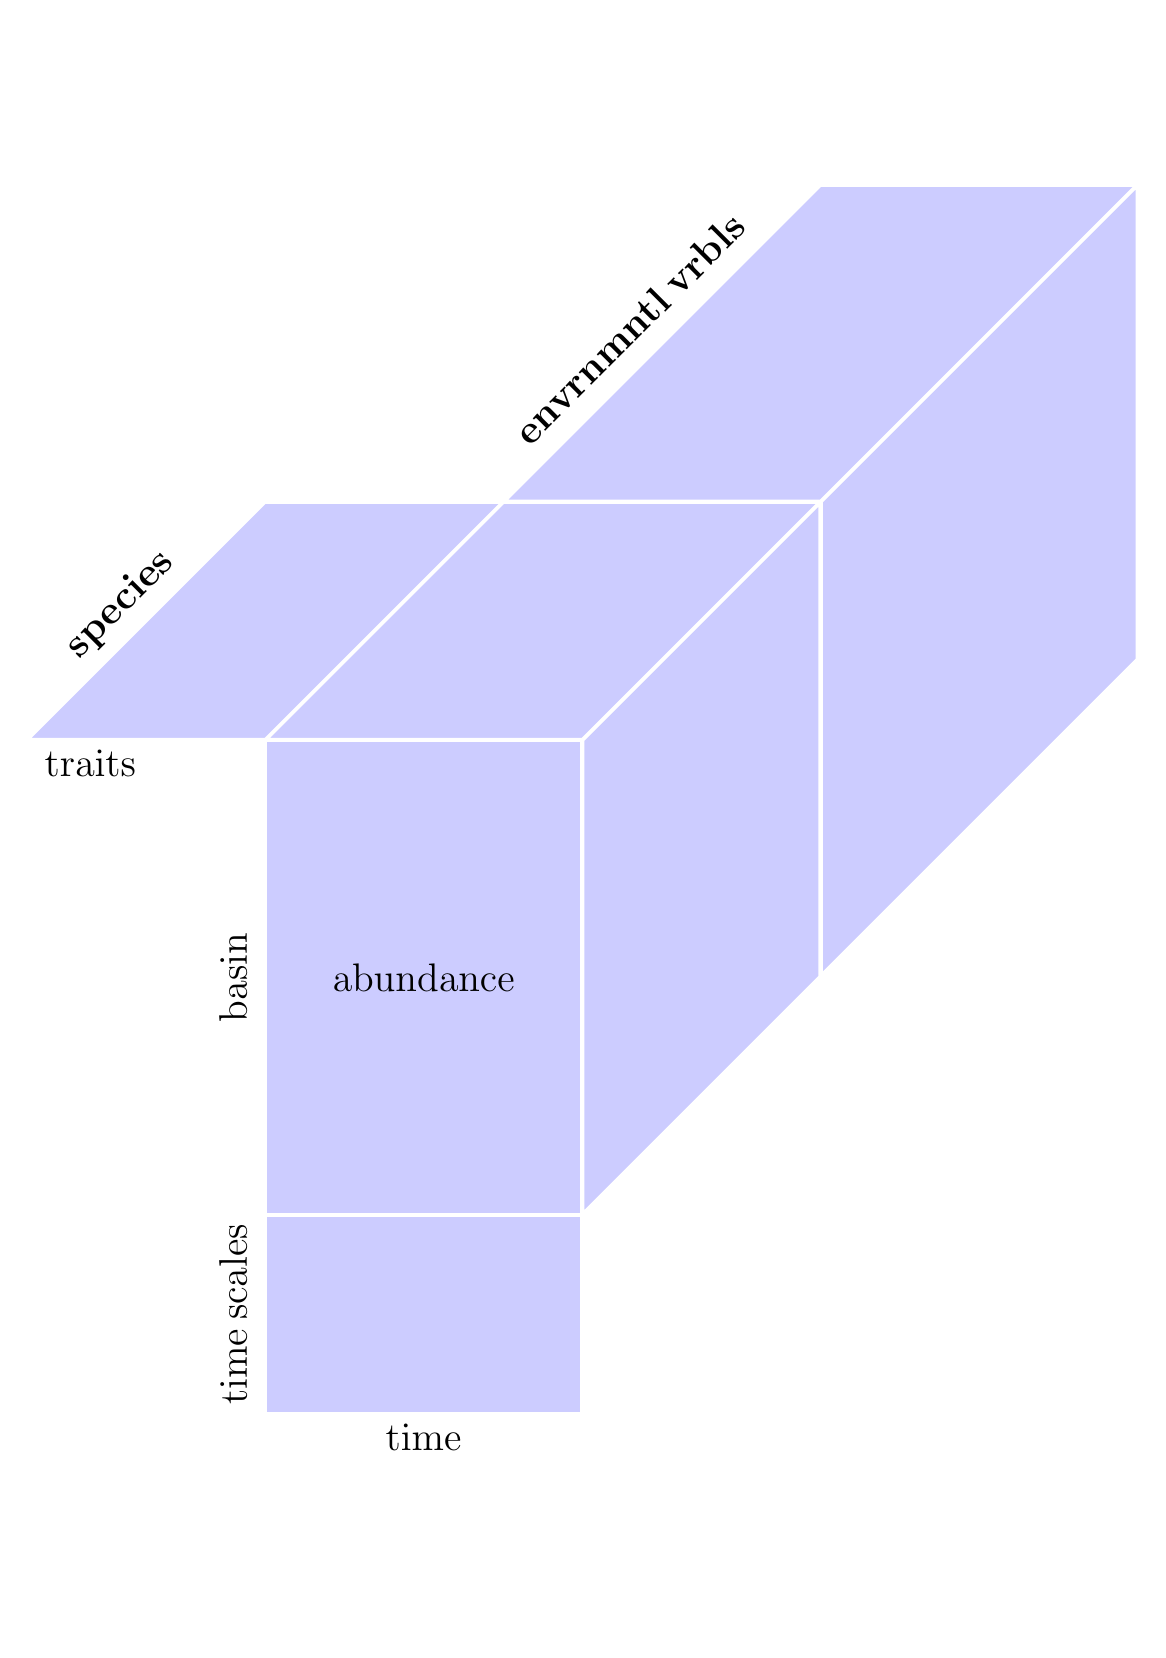
\begin{tikzpicture} [
	text centered,
	node distance=0cm,
	yfront/.style={
		rectangle,draw=blue!0,fill=blue!20,thick,
		minimum width=4cm,minimum height=6cm},
	time/.style={
		rectangle,draw=blue!0,fill=blue!20,thick,
		minimum width=4cm,minimum height=2.5cm,
		label=below:\Large time},
	ytop/.style={
		rectangle,draw=blue!0,fill=blue!20,thick,
		minimum width=4cm,minimum height=3cm,
		xslant=1},
	xtop/.style={
		rectangle,draw=blue!0,fill=blue!20,thick,
		minimum width=4cm,minimum height=4cm,
		xslant=1},
	yside/.style={
		rectangle,draw=blue!0,fill=blue!20,thick,
		minimum width=3cm,minimum height=6cm,
		yslant=1},
	xside/.style={
		rectangle,draw=blue!0,fill=blue!20,thick,
		minimum width=4cm,minimum height=6cm,
		yslant=1},
	trts/.style={
		rectangle,draw=blue!0,fill=blue!20,thick,
		minimum width=3cm,minimum height=3cm,
		xslant=1,label=below:\Large traits},
	frnm/.style={
		rectangle,minimum height=8cm,
		minimum width=0cm,draw opacity=0,
		text width=0.8cm},
	tpnm/.style={
		rectangle,minimum height=8cm,
		minimum width=0cm,draw opacity=0,
		xslant=0,text width=0.7cm}
	]
\node [place,yfront]		(front)			{\Large abundance};
\node [place,ytop]		(top)[above=of front]	{};
\node [place,yside]		(side)[right=of front]	{};
\node [place,trts]		(trts)[left=of top]	{};
\node [place,xtop]		(xtop)[above=of top]	{};
\node [place,xside]		(xside)[right=of side]	{};
\node [place,time]		(time)[below=of front]{};
\node [place,frnm]		(frnm)[left=of front]	{\begin{turn}{90}
										\Large basin
									\end{turn}
									};
\node [place,frnm]		(frnm)[left=of time]	{\begin{turn}{90}
										\Large time 
										scales
									\end{turn}
									};
\node [place,tpnm]		(tpnm)[left=of trts]	{\begin{rotate}{45}
										\hspace{-0.8cm}
										\Large
										\textbf{species}
									\end{rotate}
									};
\node [place,tpnm]		(tpnm)[left=of xtop]	{\begin{rotate}{45}
										\hspace{-2.1cm}
										\Large
										\textbf{
											envrnmntl 
											vrbls
										}
									\end{rotate}
									};
\end{tikzpicture}
\caption{The structure of the Lac Croche zooplankton community data.} 
\label{fig:beatrix}
\end{figure}

One possible solution is to develop new \R\ analysis functions---or new software packages altogether---that are specifically designed to accept several tables as input.  There has been a fair amount of work in this direction, focusing on data with a fourth-corner problem (e.g. Chessel et al. 1996; Legendre et al. 1997; Ives and Godfray 2006; Dray and Legendre 2008; Pillar and Duarte 2010; Leibold et al. 2010; Ives and Helmus 2011).  However, this work does not apply to data sets that have other more complex multiple-table data structures (e.g. zooplankton communities in Lac Croche, Fig. \ref{fig:beatrix}).  One approach to such issues would be to build new data analysis functions for each new data structure.  But such an approach is less than ideal, as it would require that new methods be learned for each new structure---it does not take advantage of the large number of tools developed within the standard \R\ framework of data frames and formulas.  The \code{multitable} package provides an alternative approach, by introducing a multiple-table generalization of data frames---called data lists---which can be analyzed with virtually any function that can be used to analyze a data frame.  Thus, instead of providing new methods of analysis, \code{multitable} provides new methods of data management.

There are several existing \R\ packages that are designed to make data management easier (e.g. \code{reshape2}; etc.??).  In particular, the \code{mefa} and \code{mefa4} packages have been developed to organize data with a slight generalization\footnote{Several community matrices---called segments---with identical dimensions are allowed in \code{mefa}.} of the fourth-corner problem.  The \code{multitable} package has much in common with \code{mefa}, but there are noticeable differences.  For example, \code{mefa} provides more extensive tools for data summarization than \code{multitable} and \code{mefa4} integrates tools for sparse-matrix computations.  On the other hand, \code{multitable} is designed to handle more general data structures than \code{mefa} or \code{mefa4} (e.g. \code{mefa} cannot organize the Lac Croche data structure, Fig. \ref{fig:beatrix}).  However, we hope that \code{mefa} and \code{multitable} will be complementary, not competitive.

The \code{multitable} model of data organization is illustrated in Figure \ref{fig:model} (\code{mefa} uses a similar model).  In blue are the elements of the standard \R\ workflow: data frames; formulas; functions; and analyses.  The \code{multitable} package seeks to facilitate the use of such workflows with multiple-table data by creating tools (arrows and red boxes) for organizing and manipulating such data.  These tools are based on a new kind of object, called a data list, which is used to organize multiple-table data.  Data lists can be manipulated much like data frames (e.g. variables can be transformed; groups of observations extracted or removed).  Our design principle was to keep the manipulation of data lists as similar as possible to the manipulation of data frames.  Once data lists are ready for analysis \code{multitable} provides tools for coercing them into data frames, thereby entering the standard \R\ workflow.  Importantly, data, formulas, and functions are kept separate, thus preserving the benefits of using \R\ in a standard way.

\begin{figure}
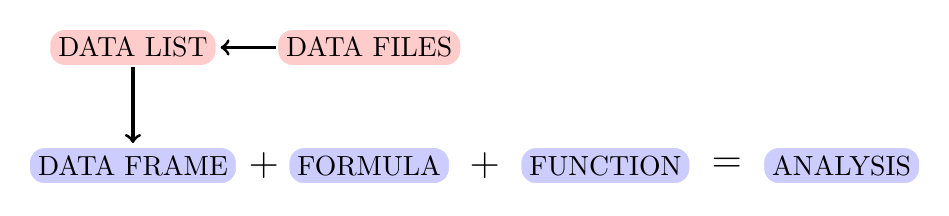
\begin{tikzpicture} [
	object stand/.style={
		rectangle,draw=blue!0,fill=blue!20,thick,
		rounded corners=2mm},
	object new/.style={
		rectangle,draw=red!0,fill=red!20,thick,
		rounded corners=2mm},
	otpt/.style={
		rectangle,draw=blue!0,fill=blue!20,thick,
		rounded corners=2mm},
	plus/.style={},
	tip/.style={
		->,shorten >=1pt,line width=0.4mm}]
\node[object new] (data files) 		at (3,1.5) {DATA FILES};
\node[object new] (data list) 		at (0,1.5) {DATA LIST};
\node[object stand] 	(data frame) 	at (0,0) {DATA FRAME};
\node[object stand] 	(formula) 		at (3,0) {FORMULA};
\node[object stand] 	(function) 		at (6,0) {FUNCTION};
\node[otpt]		(analysis) 		at (9,0) {ANALYSIS};
\node[plus] 					at (1.663,0) {\Large{+}};
\node[plus] 					at (4.47,0) {\Large{+}};
\node[plus] 					at (7.543,0) {\Large{=}};
\draw[tip] (data list.south) -- (data frame.north);
\draw[tip] (data files.west) -- (data list.east);
\end{tikzpicture}
\caption{The \code{multitable} paradigm for including multiple-table data (in red) into the standard \R\ workflow (in blue).  Data lists are used to organize and manipulate multiple-table data as a single \R\ object, even though it must be stored in multiple text-based data files.  When such data are required for analysis, they are coerced into a data frame.  Once in data frame form, they can be used in analyses by combining them with formulas (to specify hypothetical relationships between variables) and functions (to call computational methods).} 
\label{fig:model}
\end{figure}

\section{The structure of data lists}

The \code{multitable} package comes with a fictitious \code{data.list}, to illustrate how these objects work.
\begin{Schunk}
\begin{Sinput}
> library(multitable)
> data(fake.community)
> fake.community
\end{Sinput}
\begin{Soutput}
abundance:
---------
, , capybara

            2009 2008 1537
midlatitude    4    0    0
subtropical    0   10    0
tropical       8    0    0
equatorial     0    7    0
arctic         0    0    0
subarctic      0    0    0

, , moss

            2009 2008 1537
midlatitude    0    6    0
subtropical    0    0    0
tropical       9    0    0
equatorial     0    3    0
arctic         5    0    0
subarctic      0    0    0

, , vampire

            2009 2008 1537
midlatitude    0    0    0
subtropical    0    0    1
tropical       0    0    0
equatorial     0    0    0
arctic         0    0    0
subarctic      0    0    0

Replicated along:  || sites || years || species || 


temperature:
-----------
            2009 2008 1537
midlatitude   NA   10   NA
subtropical   25   20   NA
tropical      48   50   NA
equatorial    50   30   NA
arctic       -37  -30   NA
subarctic      3    0   NA
Replicated along:  || sites || years || 


precipitation:
-------------
            2009 2008 1537
midlatitude   NA   20   NA
subtropical   99  100   NA
tropical     149  150   NA
equatorial   199  200   NA
arctic        21   20   NA
subarctic     41   40   NA
Replicated along:  || sites || years || 


body.size:
---------
capybara     moss  vampire 
     140       NA      190 
Replicated along:  || species || 


metabolic.rate:
--------------
capybara     moss  vampire 
      20        5        0 
Replicated along:  || species || 


homeotherm:
----------
capybara     moss  vampire 
       Y        N        N 
Levels: N Y
Replicated along:  || species || 


REPLICATION DIMENSIONS: 
  sites   years species 
      6       3       3 
\end{Soutput}
\end{Schunk}

At first sight, this \code{data.list} object looks very different from standard \code{data.frame} objects, but on second look we can see that they are really quite similar.  Just like data frames, data lists are composed of a number of variables---in this case, we have six variables (abundance; temperature; precipitation; body size; metabolic rate; and homeotherm) each identified in the printed object above by underlined names.  The variables in data lists must be printed in this sequential manner, rather than as columns neatly lined up in a data frame, precisely because the variables in multiple-table data sets do not line up neatly; this is the problem \code{multitable} seeks to address.

Also as in data frames, the replication of variables in data lists are represented as vectors of values.  The main difference between the two objects in this regard is that the vectors that represent variables in data lists have a \code{dim} (i.e. dimension) attribute, which gives it further structure.  In \R, vectors with \code{dim} attributes are best thought of as matrices and arrays of numbers.  For example, the abundance variable is replicated along three dimensions (sites; years; and species), and therefore is a three dimensional array of data.  This information is indicated above after the variable itself is printed.  Some variables are only replicated along two dimensions (e.g. temperature and precipitation) and others only a single dimension (e.g. body size; metabolic rate; and homeotherm).  

Importantly however, although the variables are not replicated along all of the same dimensions, they do share dimensions; and it is this dimension sharing that allows us to relate variables to each other.  To appreciate the dimension sharing of this example, we can use the \code{summary} method for \code{data.list} objects.
\begin{Schunk}
\begin{Sinput}
> summary(fake.community)
\end{Sinput}
\begin{Soutput}
        abundance temperature precipitation body.size metabolic.rate homeotherm
sites        TRUE        TRUE          TRUE     FALSE          FALSE      FALSE
years        TRUE        TRUE          TRUE     FALSE          FALSE      FALSE
species      TRUE       FALSE         FALSE      TRUE           TRUE       TRUE
\end{Soutput}
\end{Schunk}
\noindent This method returns a logical table with dimensions of replication as rows and variables as columns.  A value of \code{TRUE} appears in cells corresponding to variables that are replicated along a particular dimension, and a value of \code{FALSE} appears otherwise.  We can see that the \code{sites} and \code{years} dimensions relates abundance, temperature, and precipitation; whereas, the \code{species} dimension relates abundance, body size, metabolic rate, and homeotherm.

Note that some \code{FALSE} entries are bio-physical necessities, whereas some are properties of the study design.  For example, suppose that later in the study, the researchers decided that it was necessary to get some idea of the spatial variation in metabolic rates.  It would then be possible to measure metabolic rates of the species at different sites, thereby changing the \code{FALSE} associated with the metabolic rate-sites cell to a \code{TRUE}.  To the contrary, it is physically and logically impossible to measure the precipitation of a species, and so this \code{FALSE} is necessarily \code{FALSE}.

\section{Subscripting data lists}

This structure relating variables and dimensions of replication, allows us to manipulate multiple variables simultaneously.  In particular, \code{multitable} makes it possible to extract pieces of a data list will maintaining its structure.  For example, examining the data suggests that 1537 might have been an outlying year relative to 2008 and 2009.  We can exclude data from 1537 just as we would with a single \R\ array.
\begin{Schunk}
\begin{Sinput}
> fake.community[, c("2008", "2009"), ]
\end{Sinput}
\begin{Soutput}
abundance:
---------
, , capybara

            2008 2009
midlatitude    0    4
subtropical   10    0
tropical       0    8
equatorial     7    0
arctic         0    0
subarctic      0    0

, , moss

            2008 2009
midlatitude    6    0
subtropical    0    0
tropical       0    9
equatorial     3    0
arctic         0    5
subarctic      0    0

, , vampire

            2008 2009
midlatitude    0    0
subtropical    0    0
tropical       0    0
equatorial     0    0
arctic         0    0
subarctic      0    0

Replicated along:  || sites || years || species || 


temperature:
-----------
            2008 2009
midlatitude   10   NA
subtropical   20   25
tropical      50   48
equatorial    30   50
arctic       -30  -37
subarctic      0    3
Replicated along:  || sites || years || 


precipitation:
-------------
            2008 2009
midlatitude   20   NA
subtropical  100   99
tropical     150  149
equatorial   200  199
arctic        20   21
subarctic     40   41
Replicated along:  || sites || years || 


body.size:
---------
capybara     moss  vampire 
     140       NA      190 
Replicated along:  || species || 


metabolic.rate:
--------------
capybara     moss  vampire 
      20        5        0 
Replicated along:  || species || 


homeotherm:
----------
capybara     moss  vampire 
       Y        N        N 
Levels: N Y
Replicated along:  || species || 


REPLICATION DIMENSIONS: 
  sites   years species 
      6       2       3 
\end{Soutput}
\end{Schunk}
\noindent This command returns the same data list of variables but without the data from 1537.  In particular, for every variable replicated along the \code{years} dimension is subscripted appropriately.  As another example, perhaps we want all of the data on the first species (i.e. capybara) in 1537 for the first three sites.
\begin{Schunk}
\begin{Sinput}
> fake.community[1:3, "1537", 1]
\end{Sinput}
\begin{Soutput}
abundance:
---------
, , capybara

            1537
midlatitude    0
subtropical    0
tropical       0

Replicated along:  || sites || years || species || 


temperature:
-----------
            1537
midlatitude   NA
subtropical   NA
tropical      NA
Replicated along:  || sites || years || 


precipitation:
-------------
            1537
midlatitude   NA
subtropical   NA
tropical      NA
Replicated along:  || sites || years || 


body.size:
---------
capybara 
     140 
Replicated along:  || species || 


metabolic.rate:
--------------
capybara 
      20 
Replicated along:  || species || 


homeotherm:
----------
capybara 
       Y 
Levels: N Y
Replicated along:  || species || 


REPLICATION DIMENSIONS: 
  sites   years species 
      3       1       1 
\end{Soutput}
\end{Schunk}
\noindent Notice also that for each different subset of the data, the new replication dimensions are printed after the data.

\section{Transforming variables in data lists}

Often we need to transform variables before passing data frames to functions.  This is easily done with variables in data lists as well.  For example, suppose we want to make a $\log(x+1)$ transformation of the abundance data.
\begin{Schunk}
\begin{Sinput}
> fake.community$abundance <- log(fake.community$abundance + 1)
> fake.community$abundance
\end{Sinput}
\begin{Soutput}
, , capybara

                2009     2008 1537
midlatitude 1.609438 0.000000    0
subtropical 0.000000 2.397895    0
tropical    2.197225 0.000000    0
equatorial  0.000000 2.079442    0
arctic      0.000000 0.000000    0
subarctic   0.000000 0.000000    0

, , moss

                2009     2008 1537
midlatitude 0.000000 1.945910    0
subtropical 0.000000 0.000000    0
tropical    2.302585 0.000000    0
equatorial  0.000000 1.386294    0
arctic      1.791759 0.000000    0
subarctic   0.000000 0.000000    0

, , vampire

            2009 2008      1537
midlatitude    0    0 0.0000000
subtropical    0    0 0.6931472
tropical       0    0 0.0000000
equatorial     0    0 0.0000000
arctic         0    0 0.0000000
subarctic      0    0 0.0000000

attr(,"subsetdim")
  sites   years species 
   TRUE    TRUE    TRUE 
\end{Soutput}
\end{Schunk}

\section{Simple analysis functions}

Data lists can be passed `as is' to many standard functions in \R\ that normally take data frames.  In the next section I will define this class of functions in more detail, but for now consider this simple example.  Perhaps we want to explore whether the interaction between body size and temperature has an influence on abundance.  As a first attempt at model building, we fit a linear model using \code{lm}.
\begin{Schunk}
\begin{Sinput}
> lm(abundance ~ (body.size * temperature), data = fake.community)
\end{Sinput}
\begin{Soutput}
Call:
lm(formula = abundance ~ (body.size * temperature), data = fake.community)

Coefficients:
          (Intercept)              body.size            temperature  body.size:temperature  
            1.5718991             -0.0082732              0.0477659             -0.0002514  
\end{Soutput}
\end{Schunk}
And this works just as well with mixtures of categorical and numerical data.
\begin{Schunk}
\begin{Sinput}
> lm(abundance ~ -1 + (homeotherm * temperature), data = fake.community)
\end{Sinput}
\begin{Soutput}
Call:
lm(formula = abundance ~ -1 + (homeotherm * temperature), data = fake.community)

Coefficients:
            homeothermN              homeothermY              temperature  
              0.3450914                0.4136577               -0.0004895  
homeothermY:temperature  
              0.0130595  
\end{Soutput}
\end{Schunk}
It also works with other `simple' functions, such as \code{rlm} (robust linear model) in the \code{MASS} package.
\begin{Schunk}
\begin{Sinput}
> library(MASS)
> rlm(abundance ~ (body.size * temperature), data = fake.community)
\end{Sinput}
\begin{Soutput}
Call:
rlm(formula = abundance ~ (body.size * temperature), data = fake.community)
Converged in 17 iterations

Coefficients:
          (Intercept)             body.size           temperature body.size:temperature 
         2.230510e-04         -1.173953e-06          7.435033e-06         -3.913176e-08 

Degrees of freedom: 22 total; 18 residual
  (32 observations deleted due to missingness)
Scale estimate: 1.39e-16 
\end{Soutput}
\end{Schunk}
\noindent Therefore, in many cases, data lists enter the standard \R\ workflow in exactly the same manner as data frames.

\section{Coercing data lists to data frames}

The reason that unmodified data lists can be passed to some functions that are expecting data frames, is that these functions try to coerce whatever data object they receive into a data frame.  When the \code{multitable} package is loaded, these functions can find a method for making such a conversion.  This method can be accessed by users directly via the \code{as.data.frame} function from the \R\ \code{base} package.  For example, we can pass the \code{fake.community} data to \code{as.data.frame}.
\begin{Schunk}
\begin{Sinput}
> as.data.frame(fake.community)
\end{Sinput}
\begin{Soutput}
                          abundance temperature precipitation body.size metabolic.rate
midlatitude.2009.capybara 1.6094379          NA            NA       140             20
subtropical.2009.capybara 0.0000000          25            99       140             20
tropical.2009.capybara    2.1972246          48           149       140             20
equatorial.2009.capybara  0.0000000          50           199       140             20
arctic.2009.capybara      0.0000000         -37            21       140             20
subarctic.2009.capybara   0.0000000           3            41       140             20
midlatitude.2008.capybara 0.0000000          10            20       140             20
subtropical.2008.capybara 2.3978953          20           100       140             20
tropical.2008.capybara    0.0000000          50           150       140             20
equatorial.2008.capybara  2.0794415          30           200       140             20
arctic.2008.capybara      0.0000000         -30            20       140             20
subarctic.2008.capybara   0.0000000           0            40       140             20
midlatitude.1537.capybara 0.0000000          NA            NA       140             20
subtropical.1537.capybara 0.0000000          NA            NA       140             20
tropical.1537.capybara    0.0000000          NA            NA       140             20
equatorial.1537.capybara  0.0000000          NA            NA       140             20
arctic.1537.capybara      0.0000000          NA            NA       140             20
subarctic.1537.capybara   0.0000000          NA            NA       140             20
midlatitude.2009.moss     0.0000000          NA            NA        NA              5
subtropical.2009.moss     0.0000000          25            99        NA              5
tropical.2009.moss        2.3025851          48           149        NA              5
equatorial.2009.moss      0.0000000          50           199        NA              5
arctic.2009.moss          1.7917595         -37            21        NA              5
subarctic.2009.moss       0.0000000           3            41        NA              5
midlatitude.2008.moss     1.9459101          10            20        NA              5
subtropical.2008.moss     0.0000000          20           100        NA              5
tropical.2008.moss        0.0000000          50           150        NA              5
equatorial.2008.moss      1.3862944          30           200        NA              5
arctic.2008.moss          0.0000000         -30            20        NA              5
subarctic.2008.moss       0.0000000           0            40        NA              5
midlatitude.1537.moss     0.0000000          NA            NA        NA              5
subtropical.1537.moss     0.0000000          NA            NA        NA              5
tropical.1537.moss        0.0000000          NA            NA        NA              5
equatorial.1537.moss      0.0000000          NA            NA        NA              5
arctic.1537.moss          0.0000000          NA            NA        NA              5
subarctic.1537.moss       0.0000000          NA            NA        NA              5
midlatitude.2009.vampire  0.0000000          NA            NA       190              0
subtropical.2009.vampire  0.0000000          25            99       190              0
tropical.2009.vampire     0.0000000          48           149       190              0
equatorial.2009.vampire   0.0000000          50           199       190              0
arctic.2009.vampire       0.0000000         -37            21       190              0
subarctic.2009.vampire    0.0000000           3            41       190              0
midlatitude.2008.vampire  0.0000000          10            20       190              0
subtropical.2008.vampire  0.0000000          20           100       190              0
tropical.2008.vampire     0.0000000          50           150       190              0
equatorial.2008.vampire   0.0000000          30           200       190              0
arctic.2008.vampire       0.0000000         -30            20       190              0
subarctic.2008.vampire    0.0000000           0            40       190              0
midlatitude.1537.vampire  0.0000000          NA            NA       190              0
subtropical.1537.vampire  0.6931472          NA            NA       190              0
tropical.1537.vampire     0.0000000          NA            NA       190              0
equatorial.1537.vampire   0.0000000          NA            NA       190              0
arctic.1537.vampire       0.0000000          NA            NA       190              0
subarctic.1537.vampire    0.0000000          NA            NA       190              0
                          homeotherm
midlatitude.2009.capybara          Y
subtropical.2009.capybara          Y
tropical.2009.capybara             Y
equatorial.2009.capybara           Y
arctic.2009.capybara               Y
subarctic.2009.capybara            Y
midlatitude.2008.capybara          Y
subtropical.2008.capybara          Y
tropical.2008.capybara             Y
equatorial.2008.capybara           Y
arctic.2008.capybara               Y
subarctic.2008.capybara            Y
midlatitude.1537.capybara          Y
subtropical.1537.capybara          Y
tropical.1537.capybara             Y
equatorial.1537.capybara           Y
arctic.1537.capybara               Y
subarctic.1537.capybara            Y
midlatitude.2009.moss              N
subtropical.2009.moss              N
tropical.2009.moss                 N
equatorial.2009.moss               N
arctic.2009.moss                   N
subarctic.2009.moss                N
midlatitude.2008.moss              N
subtropical.2008.moss              N
tropical.2008.moss                 N
equatorial.2008.moss               N
arctic.2008.moss                   N
subarctic.2008.moss                N
midlatitude.1537.moss              N
subtropical.1537.moss              N
tropical.1537.moss                 N
equatorial.1537.moss               N
arctic.1537.moss                   N
subarctic.1537.moss                N
midlatitude.2009.vampire           N
subtropical.2009.vampire           N
tropical.2009.vampire              N
equatorial.2009.vampire            N
arctic.2009.vampire                N
subarctic.2009.vampire             N
midlatitude.2008.vampire           N
subtropical.2008.vampire           N
tropical.2008.vampire              N
equatorial.2008.vampire            N
arctic.2008.vampire                N
subarctic.2008.vampire             N
midlatitude.1537.vampire           N
subtropical.1537.vampire           N
tropical.1537.vampire              N
equatorial.1537.vampire            N
arctic.1537.vampire                N
subarctic.1537.vampire             N
\end{Soutput}
\end{Schunk}

%Because the variables differ in the dimensions they are replicated along, replication of such multiple-table data sets cannot simply be represented as rows in a data frame without either repeating data values to fill up the resulting holes (e.g. fourth-corners) or reducing the information content of the data.

\section{Theory}

Data lists are based on a distinction between 

The \code{multitable} package  coerce multiple-table data into a single data frame?  

This model of data organization is made possible by new objects, called data lists.  These data list objects organize and relate data from multiple tables, which were stored in multiple text-based data files.  Once in data list form, handling multiple-table data is much like handling single-table data in data frames; in fact data lists are much like the data frames that you have come to love!

Like data lists 





\section{Reading multiple data files into a data list}
\section{Manipulating data lists}
\section{Simple analyses with data lists}
\section{Coercing data lists to data frames}


\end{document}
